\documentclass[12pt,a4paper,oneside, titlepage]{report}

\usepackage[utf8]{inputenc}
\usepackage[T1]{fontenc}
\usepackage[french]{babel}
\usepackage{amssymb}
\usepackage{amsmath}
\usepackage{graphicx}
\usepackage{float}
\usepackage{mathtools}
\usepackage[table,xcdraw]{xcolor}


\author{Matteo Besançon}

\title {Parallélisme \\ \large TP 6}
\date{\today}


\begin{document}

	\maketitle
	\newpage

	\section*{Introduction}
	Pour ce TP, il nous a été demandé de réimplémenter l'algorithme de Julia, comme pour le TP5, mais de façon à pouvoir l'exécuter avec CUDA cette fois-ci.

 est une plateforme de parallel computing GPU inventée par Nvidia. En effet, les GPU sont optimisés pour effectuer certains types de calcul utilisés pour faire des rendus graphiques.

	\section*{Méthode}

	Dans un premier temps, nous avons dû récrire l'algorithme de Julia afin qu'il puisse être exécuté en CUDA. Il faut noter que, contrairement à du code standard, en CUDA nous devons définir quelle partie du code s'exécute sure le host et quelle partie s'exécute sur le device.

	Pour écrire ce code nous nous sommes fortement inspiré du code de référence donné au TP précédent ainsi que des exemples CUDA disponibles ici : http://unige.ch/spc/en/info/teaching/parallelisme/programmation-sur-gpu-avec-cuda/

	Nous avons ensuite lancé ce programme sur Baobab 15 fois, avec les mêmes paramètres que le TP précédents, en mesurant le temps d'exécution ainsi que le temps d'écriture sur le host.

	Les paramètres utilisés étaient $c = 0.285 + 0.013\ i$ avec une matrice $15000 \times 20000$ et un nombre max d'itération de 5000.

	Une fois le code exécuté nous nous sommes assuré que les images ainsi créées étaient similaires à celle crée avec le code de référence.
	\section*{Résultats}

		\begin{figure}[H]
			\centering
			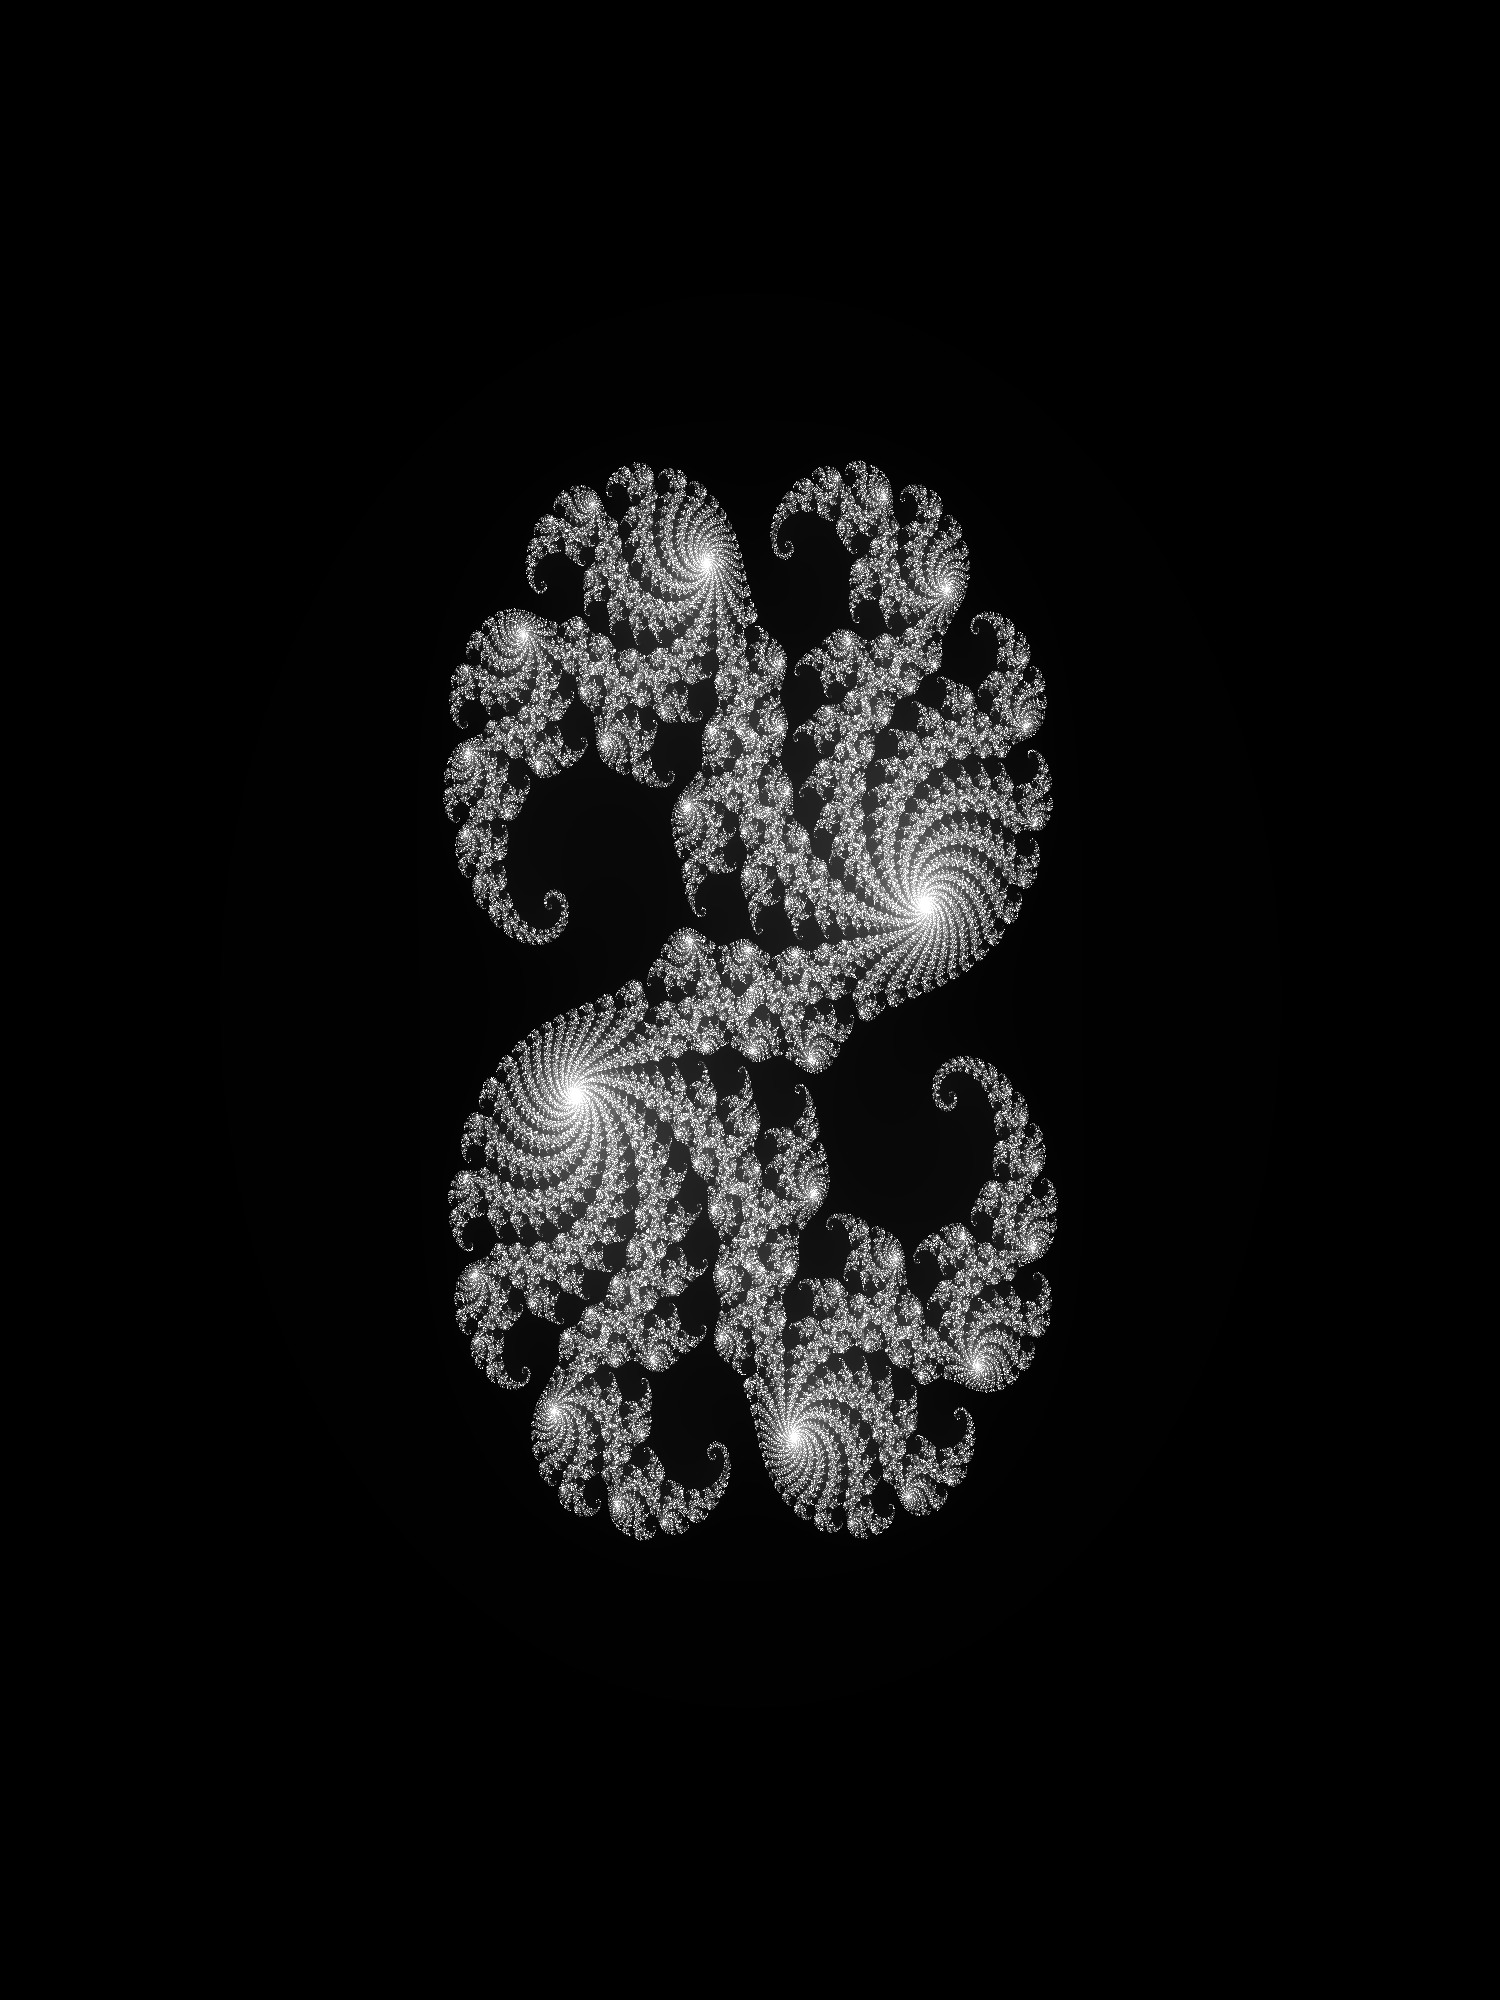
\includegraphics[scale=0.20]{../TP5/images/julia_thread_simple}
			\caption {Image d'un fractal crée avec l'algorithme de Julia en cuda (converti en JPEG)}
		\end{figure}

		Bien que l'image ait l'air similaire à celle obtenue avec le code de référence, il semble y avoir d'infimes différences, car le hash MD5 des deux fichiers ne correspond pas.

		Pour ce qui est du temps d'exécution nous avons eu les valeurs moyennes suivantes :

		Temps de calcul : 183.452 [$ms$]

		Temps de transfert : 119.188 [$ms$]

	\section*{Conclusion}

		Pour rappelle, l'exécution la plus rapide obtenue au TP précédent était de 16871.0 [$ms$] pour 120 CPUs.

		 On note tout de suite une différence très grande au niveau des performances. Cette différence peut facilement être expliquée par le fait que, contrairement à un CPU standard qui est prévu pour effectuer toutes sortes de calculs, les GPUs sont fortement optimisés pour ce type de calcul. En effet, là ou un CPU possèdes que quelques cœurs, un GPU en possède plusieurs centaines.

		 En ce qui concerne la différence au niveau du hash MD5 entre l'image de référence et celle obtenue avec CUDA, il est fort probable qu'elle soit liée à une différence de précision au niveau des calculs entre un CPU et un GPU, spécialement au niveau des variables à virgules flottantes.

\end{document}
